
\section{A software ecology}


%Software development for humanoid robots is somewhat of a back-water.
%Although it is a topic that excites the public imagination, the
%actual resources devoted worldwide are quite low.  The Japanese
%government and car manufacturers have invested in some high-profile
%projects...

%After discussing details of YARP we believe contribute to reuse,
%we'd like to step back and look at the broader picture.
%
Our initial motivation was that
many robot projects are ``black holes'', in terms of software.  A lot
of software gets sucked in, but very little comes out.  Once a piece
of software has been adapted to a particular robot, it takes a lot
of work to extricate it again and apply it to another.
%
Obviously the answer to this problem is modularity.  So there are 
now several architectures/middleware/frameworks for modular robot systems,
YARP being one of them.
The major concern for any such middleware (including YARP) should be that it not 
also become
in turn a ``black hole''~-- the
danger is that once a piece of software has been adapted
to a particular architecture/middleware/framework, it may take a lot of work to extricate it
again and apply it to another.  That would be a bit somewhat self-defeating.
%
So modularity alone is not a solution to software reuse, since 
different organizing architectures, middleware, or frameworks may be mutually
incompatible.  It is important that modules developed can fit
into a broader ``ecology'': the  complicated, sometimes messy
collection of niches world-wide in which software development occurs.

%We study YARP from this perspective.  How sticky is resultant user
%code to the robot and to the framework itself?





\begin{figure}[t]
\begin{center}
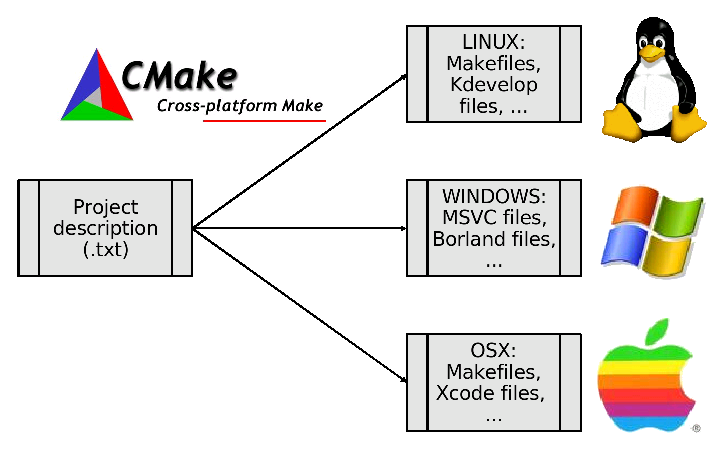
\includegraphics[height=3.5cm]{fig-cmake}
\ \ \ \ \ \ 
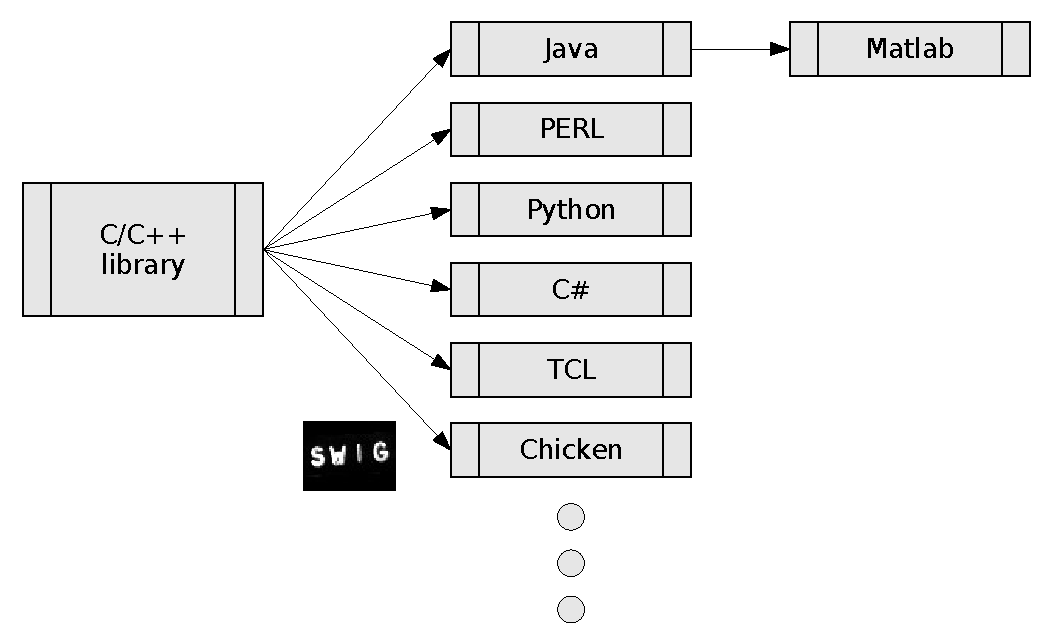
\includegraphics[height=3.5cm]{fig-swig}
\caption{
%
\label{fig:build}
%
With the aid of a set of free and open source tools, 
a C/C++ based project like YARP can have a very
wide reach.
%
C/C++ source code is quite portable and widely supported, but the
infrastructure needed to compile such programs varies a great 
deal.  Tools like autoconf and automake have smoothed over
the differences for UNIX-like systems. CMake (left) goes
further and makes projects easy to compile within a
wide range of integrated development environments
(including UNIX-like systems, but also Microsoft Visual C++,
Apple Xcode, Kdevelop, etc).
%
For operating-system dependent functions, we use the free
and open source ACE library~\cite{ACEBook}.
%
SWIG (right) takes C/C++ source code and generates ``wrappers''
for it, usable from many different languages (including Matlab
via Java).
%
%
}
\end{center}
\end{figure}




\subsection{C/C++}

We decided to use C++ as the main language for development. This 
is motivated by the fact that C++ is an object oriented language
that is widely used by many developers in the world, and is well 
supported and portable on almost all the available platforms. 
Perhaps more importantly for robotics, C++ allows writing very 
efficient code and interfacing with the hardware at the lowest 
level.
%
The drawback is that the compile process varies a lot depending 
on the platform and development environment. For example Linux 
and Cygwin developers use mostly Makefiles, whereas Microsoft Windows 
developers may prefer Visual Studio project files. 
Altough C++ has reached a fairly good level 
of portability which allows, with a reasonable effort, writing 
applications that compile on all platforms, it is still very 
common to have to wrestle to port code that was written for 
one platform onto another. On the other hand, following a 
modular approach, we would like our software to be as flexible 
as possible and be adaptable to the needs of users and the platform that 
they work on. In YARP, unavoidable dependencies 
have been made as localized as possible to modules that can be 
compiled or not depending on the underlying system and user 
choices. So for example applications that require a GUI get
compiled only when the supporting libraries
%
% (mainly GTK+) 
%
are installed on the system, and all the essential operations
of YARP are independent of GUIs.
%
%Another example is the mathematical
%library which is built on top of the GNU Scientific Library. 
%The idea is that only the modules that only and \emph{all} the 
%modules that can be compiled are actually built.
%
We take similar care for dependencies on mathematical and 
image processing libraries.
%
%To avoid asking the user to go through a tedious and long process 
%of manual configuration, a program automatically inspects the 
%system and generates the files necessary to compile YARP 
%on the host system (e.g. make files in Linux systems, or Visual 
%Studio project files in Windows). This simplifies development, 
%because it is no longer required to distribute build files 
%for all possible platforms.

Among the available tools for automatic configuraton of 
software packages, we decided to use CMake~\cite{cmake}.
CMake is a cross-platform, open-source build system. It 
produces build files for the environment of choice (e.g. 
makefiles for Unix, Borland and MinGW and project files for 
all Microsoft compilers) starting from a language independent 
description. The language of CMake is powerful enough
to support a flexible configuration process based 
on the packages that are available in the system and 
the preferences of the user (see Figure~\ref{fig:build}). Through 
CMake the build process of YARP is robust, simple and 
flexible.
%
%Has the excellent property of being simpler than making Makefiles
%or configuring a project, when external libraries are involved.
%
%The big downside is that the language is unfamiliar and a bit ugly.
%It is simple and well-documented, but quirky.  An alternative with
%some similar properties, scons, uses python instead.  The ant system
%uses with java also seems cleaner.  However, it gets the job
%done, and has the huge advantage of not being dependent on an
%external language being installed.
%
CMake is free and open-source, with a healthy community of 
developers.
%
We use another free and open-source tool called SWIG to make
YARP easy to use from many different languages.
%
In all these choices, we are following the practices of
large successful open-source projects.

%%\subsection{Repositories}
%%sourceforge.  debian.


\begin{figure}[t]
\begin{center}
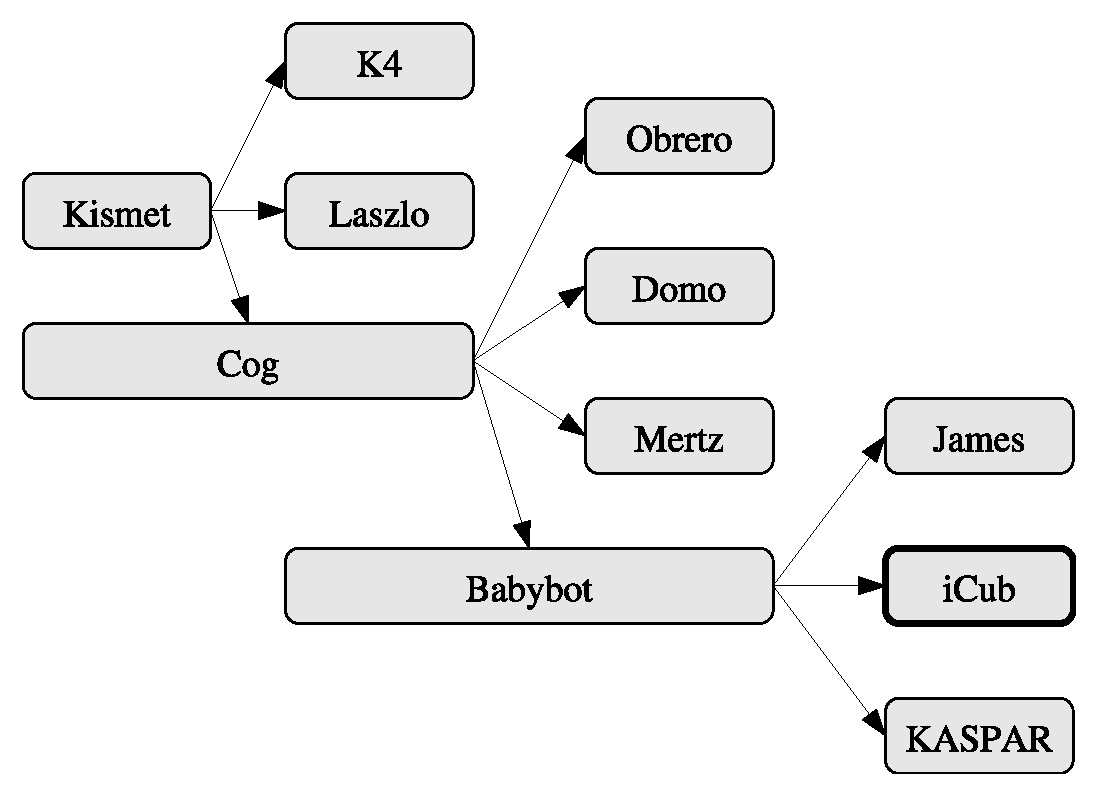
\includegraphics[height=5cm]{fig-family}
\caption{
%
\label{fig:family}
%
A potted history of YARP (for more details, see \cite{metta2006yarp}).  YARP was born on Kismet~\cite{breazeal01active},
grew up on Cog~\cite{brooks99cog} and 
BabyBot~\cite{natale05linking}, and serves as the
software architecture for the iCub humanoid \cite{tsagarakis2007icub}.
%
Along the way other humanoids have also used the system.
%
With ICub, we are trying to create some hardware ``genes''
that can travel along too, so each robot does not need to
be designed from scratch.
%
There are currently 9 copies of the ICub head.
%
%
}
\end{center}
\end{figure}



\subsection{Free Software}

The ability to integrate software modules into a system
depends not just on the technical constraints attached
to their use, but also the cultural constraints
(be they social, legal, or commercial) they carry.
%
For example, whether two modules can be integrated
can depend not just on their interfaces but also on
the conditions under which use of the modules
is permitted by their respective creators,
and what conditions the integrator wishes to 
apply to the aggregated system.  
%
This adds a great deal of complexity to the process
of integration.
%
In general, software produced under conditions where the 
creator has strong opinions about how it should be 
used, and enforces those opinions in licensing
and other measures, does not make a good module 
to build on.
%
It is possible, but painful.

The Free Software model is an alternative that strikes a different
balance between creator and integrator.  It proposes a set of standard
freedoms which should be granted with software. Taken together 
these freedoms make
the software actually useful as building blocks without excessive
social/legal/commercial complexity.  The freedoms are enforced using
copyright law principles that apply to most of the world.

The Free Software model says nothing about the cost of software,
although it does tend to contribute to commoditization, driving the
cost of infrastructure-related software such as webservers and
operating systems down.  Free software should not be confused with
``freeware''.  Freeware software is available without charge but may
have complex social/legal/commercial terms attached, and may
or may not grant the freedoms associated with free software
(usually not).

The effectiveness of free and open software is 
becoming better understood from a business
perspective \cite{vonkrogh2006promise}.
%
The free and open model has had a crucial 
effect in the field of embedded devices,
a large and growing market that overlaps
with robotics, spurred by the existence
of embedded Linux \cite{henkel2006selective}.
%
We release all our work under free and open licenses, in order to
encourage their use as building blocks.  Historically, our ``YARP''
software grew and developed this way, principally through a
collaboration between robotics groups at MIT and the University of
Genoa (Figure~\ref{fig:family}).



%% Has the revolutionary benefit that the user is not trapped in the role
%% of being a ``consumer'' of software, but can also be a publisher of
%% the changes, additions, and integrative work they do in an effective
%% form.  This is achieved by explicitly granting far more rights to
%% users than they have under the law of most countries, contrasting with
%% agreeably with the formerly more common practice of attempting to
%% minimize user rights.  These rights are typically granted
%% conditionally; a user may only make use of these extended rights if
%% (for example) distributed code is always available in its most useful
%% original (source) form, with compatible freedoms attached to it.  This
%% condition seeks to balance freedoms of individuals versus benefit to
%% the group.  The existence of code in usable form with freedoms 
%% attached can benefit many people;

%%The freedom to distribute code in obscure (compiled) forms



%%Split between people who emphasize pragmatic concerns and those
%%who emphasize freedom.  Just cite the issue, no need to revisit
%%it here.





\subsection{Interoperating}

The closest project in spirit to YARP is that of the Player project
\cite{vaughan2006reusable}.  
%
%We take the Player project as an example here of
%how YARP can interoperate with other architectures/frameworks.
%
The Player/Stage software collection is 
widely used in the field of mobile robotics, and is the nucleus of
a healthy, pragmatic community of developers.  
%
YARP and Player were developed
independently in different robotics communities (humanoids and mobile
robots respectively) over a similar time period.  Both over time
became open source projects; Player was registered on sourceforge (a
commonly used repository for open software) in 2001, and YARP in 2002.
Initially there was little overlap or mutual awareness between the
projects.  In 2005, YARP began refactoring its device API, influenced 
by a Player paper on this topic \cite{vaughan2003device}.
At about the same time, Player's networking was refactored to be
more flexible (``Player 2.0'', see \cite{collett2005player}) in 
order to break out of a client/server communication model and
allow a more flexible network and transport choices -- an area where 
YARP has historically been strong.  

Culturally, Player is biased towards mobile (wheeled) robots, with
sensing and algorithms for navigation being of central importance,
while YARP is biased towards humanoid robots, where there are many
loosely coupled behaviors involving different sets of sensors and
actuators.
%
In our opinion (speaking of course just for ourselves, and not the
Player developers), both projects are now at a state where if either
project had existed in mature form before the other was started, the
other could most certainly have been built by extension rather than 
separate development.
%
To make YARP, Player would need to have its device and networking
model decoupled further, its networking model and transport interface
generalized yet again, and have some new drivers developed; to make
Player, YARP would need to have many new devices developed, its use of
ACE and some C++ features excised, and many localization and mapping
related algorithms added.
%
The extensions would be quite a bit of work, but
certainly less than beginning from zero.
%
So what should we say to a new researcher starting a project and not
sure which to use?
%
How bad is it to be faced with a choice of systems rather than
a single coherent one?

%
%This is an interesting case to consider for interoperability.  YARP
%and Player are two open-source projects with relative strengths and
%weaknesses; what happens
%

The free software ecology contains many cases of long term
side-by-side projects with somewhat different cultures and goals.  We
see diversity at every level: the operating system (GNU/Linux,
FreeBSD, etc.), the desktop environment (Gnome, KDE), the command-line
shell (bash, tcsh, etc.), and so on.  When licensing permits it, code
flows quite freely from project to project.  In any case, the projects
are mutually visible, in terms of source code, mailing lists,
documentation etc.  There is duplication of effort, but in the long
run there is a growing consensus that this diversity is proving
healthy.  Since choice and change at every level is expected,
individual parts tend to be more modular and robust than they would
otherwise be in a ``monoculture.''

Ideally, with free and open software, the software ``genes'' (abstract
programmer interfaces, protocols, actual implementation code, etc.)
in different projects can flow back and forth or be aggregated.
Useful genes will tend to be picked up, less useful genes will tend to
languish.  Software trapped behind proprietary or otherwise-awkward
licenses is unlikely to survive the death of the organization it
belongs to.

It is instructive to look at two instances of YARP/Player aggregation:

\begin{itemize}

\item
Since 2006, Player contains a ``yarpimage'' driver which can accept
images from a YARP Network (see \cite{}).
%(driver written by Radu Bogdan Rusu BETTER ADD A CITATION HERE TO A WEBPAGE PERHAPS).
The motivation for the driver was that YARP can transmit
data using multicast, a transport not implemented in Player. 
This driver let Player treat YARP as a camera, just like
any of the other more regular cameras it already had drivers 
for.

\item
Since 2007, YARP contains a ``stage'' driver which gives access to 
a 2D robot simulator associated with the Player project 
from a YARP Network.  This driver let YARP treat Player/Stage as
a motor control system, just like any of the other more regular 
control boards it already had drivers for.

\end{itemize}

These instances have the property that they ``scratched an itch'' --
they met a need that a particular developer had.
They also have the property that the impact each system
has on the other is well-localized, to a single module.
%This is possible because
Much deeper integration would be possible, but already
just by being free and open source the projects can get along
for any developer who needs something from both.

In the redesign of YARP's device approach, active steps were
taken to reduce the coupling between devices and networking.
%
This was motivated by general concerns of modularity, and also
to make it simpler to take YARP devices, rip them out
of the YARP library, and use them in other projects.
%
%Rudimentary interoperability is possible between these projects
%at the device level.
%
%In fact devices have some similarity in structure between YARP and
%Player, but have the crucial difference (at least to our eyes) that
%
YARP device framework mandates a very thin C++ wrapper which permits direct function
calls, rather than forcing operation through a message passing
framework.  The value added by YARP's wrapper is to simplify the
externalization of device configuration (Player has an equivalent of
this) and to factor the device into interfaces corresponding to
different device families (which is just good software engineering,
shared by any good implementation of a hardware abstraction layer).
%
The key extra value added by YARP is to stop precisely there.
%
When writing a driver for a particular device, we make no assumptions
about how it will be communicated with (this is an area in which YARP
differs from Player).  There is no mention of message queues, 
buffering, etc., unless the device already has such things internally.

It seems strange to claim that {\em not} doing something adds value.
But this is the fundamental point of modularity, to refrain from 
making a dependency if you can avoid it.

The reason why one might want to intertwine devices and networking
is to achieve the important ability to control and monitor a device 
remotely.  For YARP, this ability is implemented at the 
{\em device family} level rather than the level of individual devices.
We provide proxy devices that can wrap any devices belonging to
a given family (such as cameras or motor control boards) and make 
them accessible remotely.  These proxies use YARP networking, but
there's nothing to stop someone else writing Player proxies, or 
proxies for standard RPC-based systems.

% (although that message passing can now be internal rather
%than across a network).
%
%In principle, YARP devices should be easy to wrap up systematically
%and efficiently for Player (since no assumptions are made about the
%communication model), but the other direction is not so easy.
%


%% The driver mechanism in both projects gives a very straightforward way
%% to integrate quickly with what could otherwise be incompatible
%% middleware.
%% %
%% At a higher level of potential interoperation, both projects are free
%% and open source, they both have documented network protocols, both have
%% made an effort to allow different transports, and both 
%% are reasonably portable.  So
%% a determined individual will probably be able to make them work
%% together on any given task.
%% %
%% Neither YARP nor Player is aimed at users unwilling or unable to
%% program.  Such users benefit from these projects indirectly, through
%% for example the ICub platform, which is being built using YARP to
%% support users from different disciplines including neuroscience
%% and experimental psychology.


%% It is an interesting question whether a higher level
%% convergence is possible.
%% %
%% %
%% From the YARP perspective, there doesn't seem any compelling reason to
%% do so right now; individuals who've needed parts of both systems have
%% been able to do so through the driver mechanisms.
%% %
%% From the Player perspective, YARP's dependence on ACE is probably
%% undesirable, and YARP uses some C++ features considered
%% undesirable in the C-with-Classes
%% style of Player (which is probably a better idea for portability).
%% Also, we use different build machinery (autotools versus CMake).
%% %
%% Due to recent changes in Player, communications could probably be
%% adapted with some work.  
%% %
%% In the next section, we look more closely at YARP's device model.
%% %


%%serialization / message passing

%%Player's communication model,
%%which used to be client/server, has recently been expanded to
%%be more flexible, and seems to be getting closer to a peer-to-peer
%%mechanism such as YARP.



%%Categories from \cite{collett2005player}:


